

%\section{Introduction}

Following the signing of the global agreement at the Paris Climate Conference in 2015, Israel set long-term goals to reduce greenhouse gas emissions in an effort to take part in the global action against climate change. Since the discovery of substantial offshore gas fields off the coast of Israel, Natural Gas (NG) has become the main fuel for electricity production in the country. In order to reduce Israel's carbon footprint, a decision has been made to close both major coal-fueled power plants at Hadera and Ashkelon in the future, and to convert them to gas fueled units. Apart from  renewable energy, this will render NG as the sole source of energy for electricity in the country. The Ministry of Energy plan is aimed at fulfilling Israel’s role in the agreement and at promoting an efficient, green economy. The objective is to generate up to 30\% of electricity using renewable energy by 2030, and potentially generate up to 100\% of electricity this way by 2050. The increasing share of renewable energy presents several challenges in the interim however, particularly with regard to the effects on the natural gas system, which must balance the intermittent and variable electricity production of uncontrollable renewable sources.

As of 2020, more than 50\% of Israel's electricity is produced from NG. The yearly demand for NG recently increased beyond 11 billion cubic meters (BCM). During the transition to the 2030 goal, that share is expected to increase up to 80\%-85\% in certain years. Moreover, two agreements were signed with Egypt and Jordan stipulating that Israel will export 130 BCM of NG from the Leviathan and Tamar gas fields over the next ten years. (At the moment, the non-electricity end use of NG in Israel is small, amounting to around 9000 MMBTU/h or around 10\% of the hourly typical flow).
Those data show that there are many issues surrounding the NG network in Israel over the next decade.

\href{https://www.noga-iso.co.il/en/}{NOGA}, Israel Independent System Operator (IISO), is the newly founded Israeli Electric System Operator. Its mandate is to act to ensure continuous electricity supply, at the required reliability and quality level, to all electricity consumers, in normal and emergency system conditions, and to manage the wholesale electricity market operations competitively and equitably. In addition to managing day-to-date operations, IISO is also in charge for planning development of the generation system, including recommendations for the required generation and storage capacity, maintaining optimal mix, location and timing for integration of generation and storage facilities. IISO is tasked to set up %In addition, setting 
criteria for planning the development of the generation system. The company mandate also includes many other aspects of the transmission system planning, such as related to data forecast, transformer placement and characterization and, overall, formulation of a multi-year plan for the transmission system development. It is recognized, that to achieve all the goals IISO needs state-of-the-art tools to model the Natural Gas system and its interaction with the Electricity network.


%\misha{Jean, Lilah, Igal  -- do we need to describe what are responsibilities of NatGas (operator of NG) add clarify relations between IISO and NatGas (coordination) in couple of sentences?}\jean{To be honest, I think we may remove all the paragraph about NOGA, which is not very relevant for the paper}\igal{I think we should keep the NOGA part. It explains in basic our interest in this work, if we add about natgaz then we have to explain the relations between to companies and this will divert the interest from our main work}

\begin{figure}
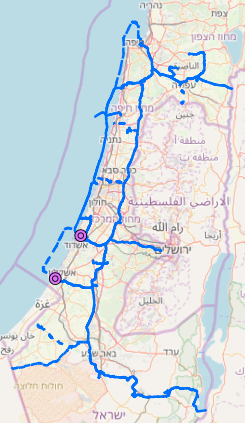
\includegraphics[width=0.33\linewidth, valign=t]{figs/fullModel.png}%
\includegraphics[width=0.33\linewidth, valign=t]{figs/reducedModel.png}%
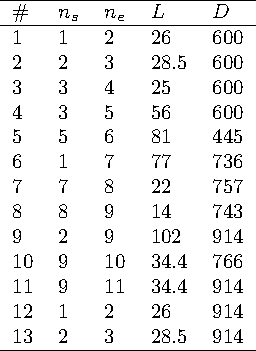
\includegraphics[width=0.33\linewidth, valign=t]{figs/pipeDescription.pdf}
\caption{
Description of the Israeli gas system: (left) Sketch of the true system. (center) Map of the reduced 11-node system that we use for this study. (right) List of pipelines in the simplified system. Their start node ($n_s$), end node ($n_e$), length $L$ in km, and diameter $D$ in mm. %\laurent{Can we mention nominal values such as max injection at bus \#1 and \#8?. I would also given nominal linepack values and then use percentages in the plots.}
\label{fig:map}
}
\end{figure}

\begin{comment}
    

\begin{figure}
    \centering
    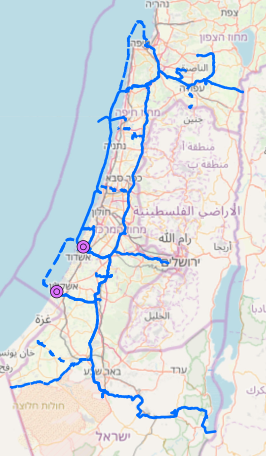
\includegraphics[width=0.35\linewidth]{figs/ScenarioResults/small_gas_map.png}%
    \includegraphics[width=0.25\linewidth]{figs/ScenarioResults/reducedModel.png}
    \caption{Comparison of the actual and reduced models of the NG network of Israel.}
    \label{fig:network}
\end{figure}


\begin{table}[] 
 %   \begin{center}
    \begin{tabular}{rr}
    \hline
           \# & Height (m)\\
           \hline
         1 & 1\\
         2 & 65\\
         3 & 140\\
         4 & 0\\
         5 & 361\\
         6 & -371\\
         7 & -55\\
         8 & 0\\
         9 & 130\\
         10 & 0\\
         11 & 175\\
         
         \hline
    \end{tabular}
%    \end{center}
%    \caption{Caption}
 %   \label{tab:my_label}
%\end{table}
%    \begin{center}
    \begin{tabular}{rrrrr}
    \hline
           \# & Start & End & Length (km) & Diameter (mm)\\
           \hline
         1 & 1 & 2 & 26 & 600\\
         2 & 2 & 3 & 28.5 & 600\\
         3 & 3 & 4 & 25 & 600\\
         4 & 3 & 5 & 56 & 600\\
         5 & 5 & 6 & 81 & 445\\
         6 & 1 & 7 & 77 & 736\\
         7 & 7 & 8 & 22 & 757\\
         8 & 8 & 9 & 14 & 743\\
         9 & 2 & 9 & 102 & 914\\
         10 & 9 & 10 & 34.4 & 766\\
         11 & 9 & 11 & 34.4 & 914\\
         12 & 1 & 2 & 26 & 914\\
         13 & 2 & 3 & 28.5 & 914\\
         
         \hline
    \end{tabular}
%    \end{center}
\caption{ Characteristics of the pipes in the reduced NG model of  Israel gas built based on the publicly available data. Left table: list of nodes. Right table: list of pipes.\label{tab:network}}
\end{table}
\end{comment}


\begin{figure}
    \centering
    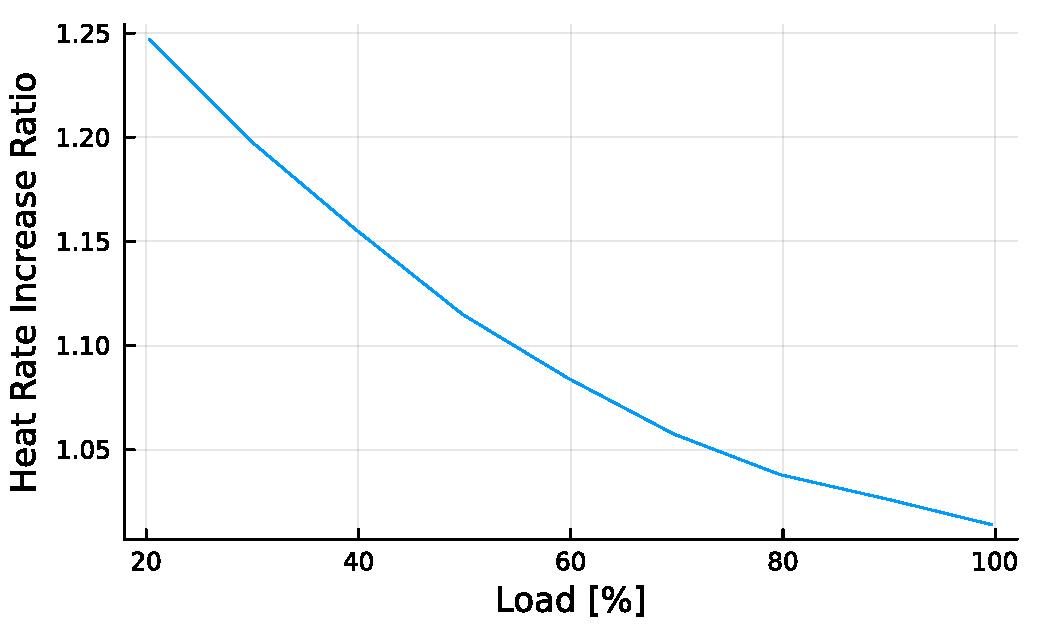
\includegraphics[width=0.75\linewidth]{figs/gas_eff_curve.pdf}%
    \caption{Typical Gas Turbine Efficiency Curve}
    \label{fig:efficiency}
\end{figure}
\begin{comment}
\misha{Jean,  this is placeholder for you to describe how the small Israel gas model was designed (main principles,  consideration, data) ... we may then extend https://www.overleaf.com/project/62bcac86d725d66a393e3f01it to building medium/large models and also to building respective power system models of Israel with a clear cross-links between the two infrastructures (see also discussion below) ...}
We have built a model for Israeli gas system based purely on public data available on the Internet.
The data source is the website of the Israel Natural Gas Authority www.ingl.co.il.
We have in fact built two models:
\begin{enumerate}
    \item A simple toy-model which comprises 11 nodes and 12 pipes; we will present this model thoroughly in this report
    \item A more detailed model (XX nodes and YY pipes) which will be discussed in the next report
\end{enumerate}
\end{comment}
%The model that we have built for Israeli gas system is based solely on public data available on the Internet.
In this manuscript we present a reduced, schematic gas model of Israel based on open-source public resources, shown in Figure \ref{fig:map}. The data source is the website of the Israel Natural Gas Authority www.ingl.co.il.
In order to perform the simulations, we need to create time series of the gas withdrawals at the model nodes. To do this, we use public data published by the Electricity Authority from the website \url{https://www.gov.il/he/departments/general/hovatdivuahnetunim}. The data are in the form of half-hourly time series of electricity production (in MW) at all units. We convert the power data to gas consumption with the help of typical gas turbines efficiency curves (see Figure \ref{fig:efficiency} for an example of such a curve). 